\documentclass[10pt]{article}

\usepackage[T1]{fontenc}
\usepackage[utf8]{inputenc}
\usepackage{lmodern}
\usepackage[margin=0.7in]{geometry}
\usepackage{microtype}
\usepackage{enumitem}
\usepackage{booktabs}
\usepackage{tabularx}
\usepackage{array}
\usepackage{graphicx}
\usepackage{float}
\usepackage{xcolor}
\usepackage{titlesec}
\usepackage[font=footnotesize, labelfont=bf, skip=3pt]{caption}
\usepackage{xurl}
\usepackage[colorlinks=true, linkcolor=black, urlcolor=blue!60!black, citecolor=black]{hyperref}

% Same compact layout as the proposal
\setlist{itemsep=0pt, topsep=1pt, parsep=0pt, leftmargin=1.4em}
\setlength{\parskip}{3pt}
\setlength{\parindent}{0pt}
\setlength{\intextsep}{5pt}
\titleformat*{\section}{\normalsize\bfseries}
\titleformat*{\subsection}{\small\bfseries}
\titlespacing*{\section}{0pt}{5pt}{0pt}
\titlespacing*{\subsection}{0pt}{4pt}{0pt}
\newcolumntype{Y}{>{\raggedright\arraybackslash}X}

\begin{document}

\begin{center}
  \vspace*{-2.2em}
  {\Large\bfseries Player Archetypes in Competitive Disc Golf}\\[3pt]
  {\large\bfseries Halfway Check-In: CSYS 6870 Data Science II}\\[3pt]
  Luc Cohen-Wanis \quad$\cdot$\quad Fall 2026
\end{center}
\vspace{-0.4em}

% ---------------------------------------------------------------------------
\section{Introduction}

The goal of this project is to use Vermont competitive disc golfer hole scores, Disc Golf Vermont Tour (DGVT) players specifically, to identify competitive disc golf play styles and hopefully archetypes. Each player has a PDGA rating, which tells you roughly how good they are, but not how they get to their score. Figure~\ref{fig:tied} is an example from this season. Four players in MA2, myself included, shot 128 at the Cold Hollow Classic in September. Relative to my own average, I gained more than a stroke a round on the one long par 4 but lost about half a stroke on each of the six long par 3s. Forrest Dodds picked up his strokes on the medium par 4s and the par 5, and Bobby Martino was close to even on every kind of hole.

The research question: \textbf{Do competitive disc golfers fall into distinct playing styles beyond overall skill, and do those styles explain and predict how players score on different kinds of holes?}

The project has three parts. The descriptive part builds a style profile for each player and clusters the profiles. The explanatory part estimates whether the effect of hole type on strokes gained depends on style. The predictive part tests whether knowing a player's style helps predict their hole scores beyond rating and hole difficulty. This check-in covers the first part. I've collected and cleaned the data, built the hole level features, and run a first round of clustering. So far the clusters look less like distinct archetypes and more like a single steady-versus-volatile dimension. I go through why below, and what that means for the rest of the semester.

\begin{figure}[H]
\centering
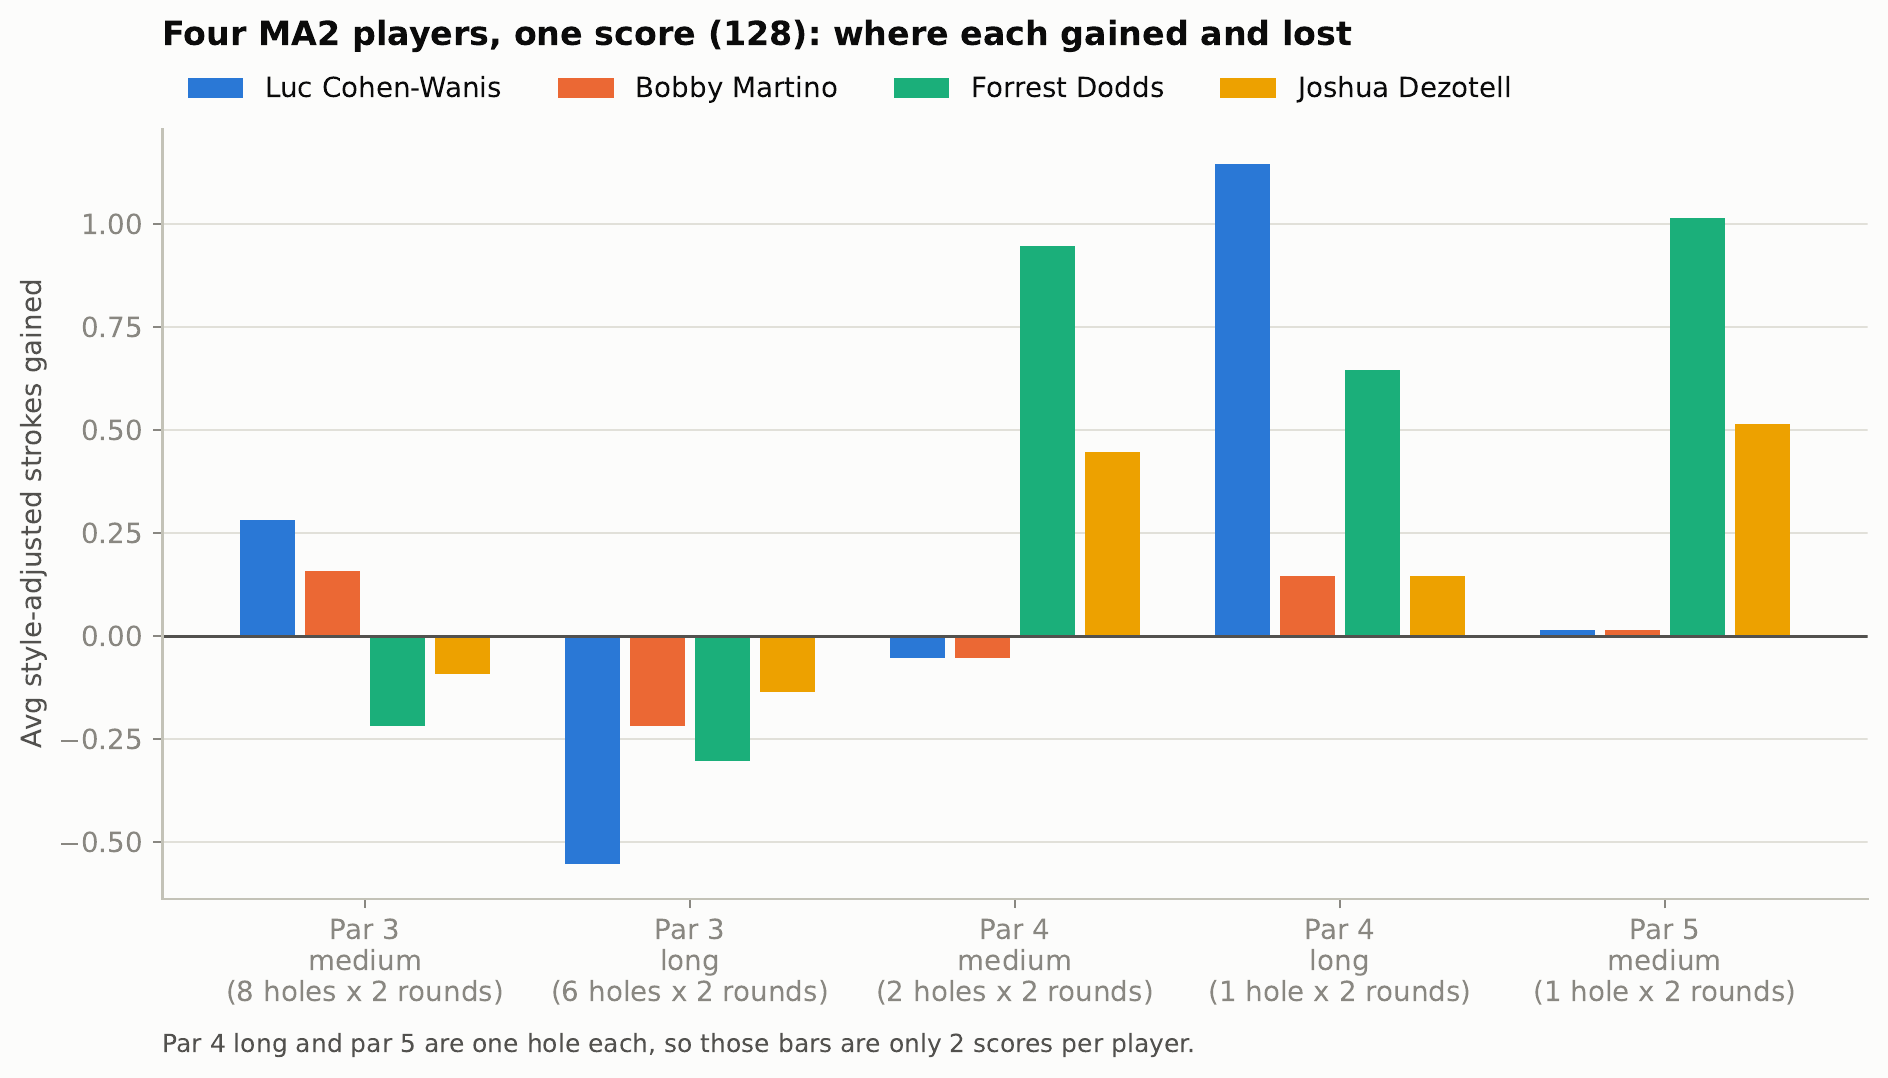
\includegraphics[width=0.62\textwidth]{figures/cold_hollow_MA2_tied_128.png}
\caption{Four MA2 players who all shot 128 over two rounds at the 2026 Cold Hollow Classic (DGVT \#11, Long layout). Each bar is a player's average style-adjusted strokes gained (Section~\ref{sec:methods}) on one par $\times$ length type. The long par 4 and the par 5 are a single hole each, so those bars are only two scores per player. That noise is why the profiles pool across many events.}
\label{fig:tied}
\end{figure}

% ---------------------------------------------------------------------------
\section{Data}

\subsection{Source and collection}

I scraped hole by hole scores from PDGA Live for every DGVT event from 2019 to 2026. I put together the event list by hand. It has 93 events with their PDGA IDs, and two of them (2022 \#11 and 2023 \#9) were cancelled. The scraper (\texttt{dgvt\_styles/scrape.py}) calls the PDGA Live JSON API directly and takes ratings from each event's results page.

The raw JSON gets parsed into four tables per season (\texttt{events}, \texttt{holes}, \texttt{rounds}, \texttt{hole\_scores}). I then wrote individual scripts to combine the seasons, run data quality checks, and build the feature table. The unit of analysis is one player on one hole in one round.

\subsection{Cleaning and quality checks}

\begin{itemize}
  \item \emph{Usable rounds.} I only use a round if every hole has a score and the hole scores add up to the round total. No scored round in any season fails the second check. Unfinished rounds show up with a score of 999 while still being marked completed, so I flag those as unusable.
  \item \emph{Layouts, not rounds or divisions.}  A round usually has more than one layout (different tees for different divisions), and each layout is usually shared by several divisions. Par, length, and field averages are computed per layout id, so a hole is only compared with others who played the same tees, and the field includes every division on that layout.
  \item \emph{Unrated players.} About 9\% of hole scores are from players with no event-time rating: 1,222 player-rounds from players with no PDGA number, and 1,333 from players who had a number but weren't rated yet. I keep them in the field averages since they were part of the field everyone else played against. I leave them out of the profiles and models.
  \item \emph{Missing hole lengths.} About 1.4\% of hole scores, mostly from a few early courses, have no hole length. Those holes don't get a hole type but are used everywhere else.
\end{itemize}

\subsection{Coverage and the 2020 start}

Table~\ref{tab:coverage} shows coverage by season. In 2019 only 2 of the 8 events have hole by hole scores, and one of those two only has them for about half the player-rounds. Since 2019 data was so sparse, I decided to ignore it and start the analysis in 2020. I keep the 2019 rows in the combined tables for reference but leave them out of every feature and model. From 2020 on nearly every event has hole scores. The exceptions are one 2020 event at 48\% coverage and one 2021 event at 2\%.

\begin{table}[H]
\centering
\footnotesize
\setlength{\tabcolsep}{6pt}
\renewcommand{\arraystretch}{0.92}
\caption{DGVT coverage by season. ``Event-time rating'' is the share of players with a PDGA number who were rated when the event was played. Cancelled events aren't counted.}
\label{tab:coverage}
\begin{tabular}{@{}lrrrrrr@{}}
\toprule
\textbf{Season} & \textbf{Events} & \textbf{With hole scores} & \textbf{Player-rounds} & \textbf{Usable rounds} & \textbf{Hole scores} & \textbf{Event-time rating} \\
\midrule
2019 & 8  & 2  & 1,376 & 179   & 3,237  & 95\% \\
2020 & 9  & 9  & 1,616 & 1,503 & 27,126 & 84\% \\
2021 & 13 & 13 & 3,543 & 3,301 & 59,452 & 90\% \\
2022 & 15 & 14 & 4,029 & 3,990 & 71,834 & 95\% \\
2023 & 12 & 11 & 3,928 & 3,867 & 69,624 & 94\% \\
2024 & 12 & 12 & 3,881 & 3,839 & 69,206 & 96\% \\
2025 & 12 & 12 & 3,500 & 3,428 & 61,776 & 98\% \\
2026 & 12 & 12 & 3,767 & 3,731 & 67,207 & 98\% \\
\bottomrule
\end{tabular}
\end{table}

The 2020--2026 feature table has 425,862 player $\times$ hole scores, from 23,659 usable player-rounds, 2,108 players, 82 events and 249 layouts. My plan is to define styles using only 2020--2023 (195,570 usable, rated hole scores) and hold out 2024--2026 for the explanatory and predictive parts. The thinking here is that this way a style is never tested on the same scores used to assign it.

% ---------------------------------------------------------------------------
\section{Methods}
\label{sec:methods}

\subsection{Hole level features}

\textbf{Strokes gained.} I borrow the strokes gained idea from golf [1], but at the hole level instead of the shot level. A player's strokes gained on a hole is the field's mean score on that hole minus the player's score. The field is everyone who played that hole on that layout in that round, across all divisions and including unrated players. The median field size is 87.

\textbf{Style-adjusted strokes gained.} This subtracts the player's own average strokes gained for the round. It takes out overall skill and how well they played that day, so what's left is where in the round they gained and lost strokes. For each player-round these values sum to zero.

\textbf{Hole type and difficulty.} Hole type is short, medium or long, using length terciles within each par. I compute the cutoffs over unique layout $\times$ hole combinations so courses that hosted lots of events don't pull them around. For par 3s the cutoffs are 225 and 294~ft. I measure difficulty separately as \texttt{field\_avg\_to\_par}, the field's average score to par on the hole in that round. In the proposal I noted that two par 4s of similar length can score very differently, and Figure~\ref{fig:length} shows that holds across the whole tour. Length and difficulty correlate at about 0.44 overall and 0.29 to 0.40 within each par, so I keep them as separate features.

\begin{figure}[t]
\centering
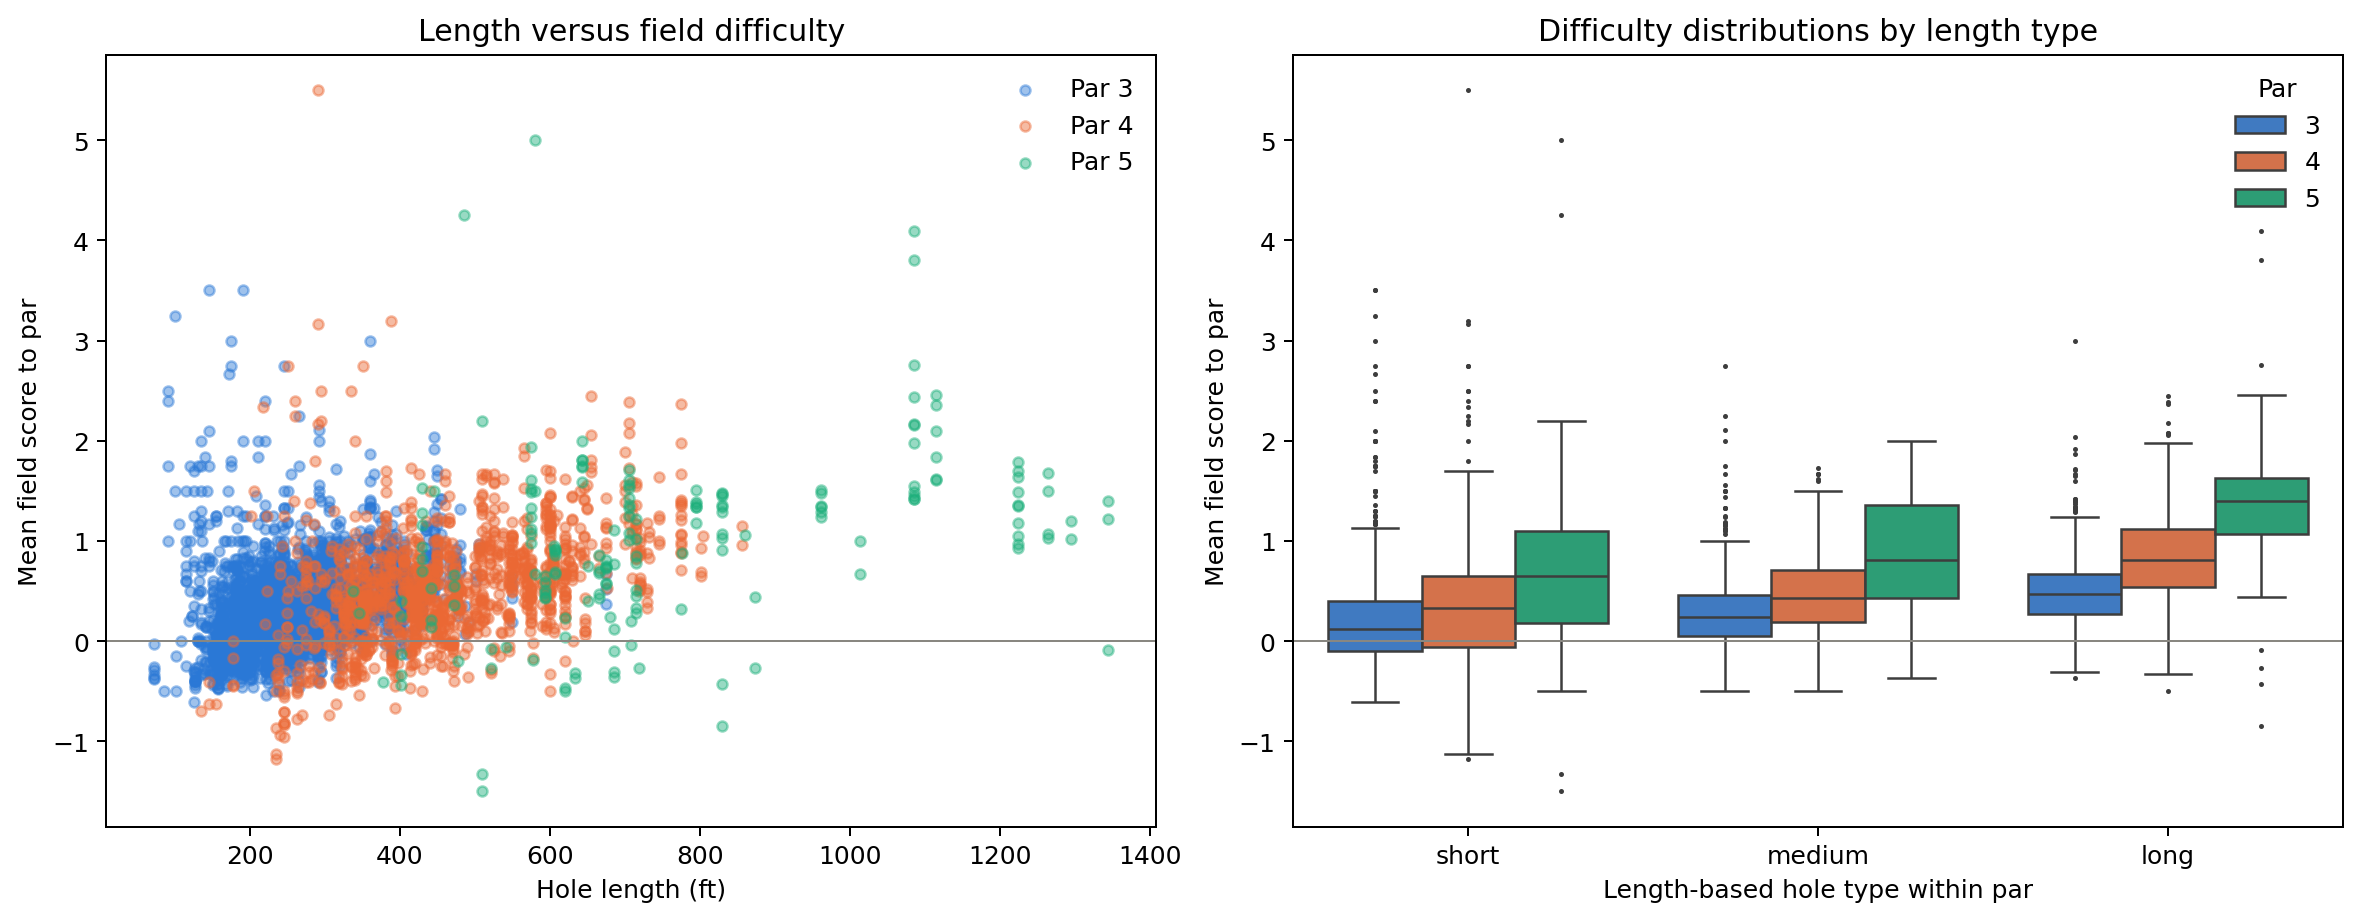
\includegraphics[width=0.85\textwidth]{figures/eda_length_vs_field_difficulty.png}
\caption{Hole length versus field difficulty for every layout hole, 2020--2026. Left: mean field score to par against length, by par. Right: difficulty by length tercile within par. Longer holes play harder on average, but there's a lot of overlap between length types.}
\label{fig:length}
\end{figure}

\subsection{Player style profiles}

Each player's profile comes from their usable, rated scores in 2020--2023 and has ten features in three groups:
\begin{enumerate}
  \item \emph{Strokes gained by hole type:} average style-adjusted strokes gained on short, medium and long holes, plus par 3s minus par 4s and 5s. I shrink each average toward zero as if the player had 50 extra holes at zero, so someone who has only played a handful of long holes doesn't get an extreme value.
  \item \emph{Score mix:} the share of holes that were birdie or better, par, bogey, and double bogey or worse.
  \item \emph{Consistency:} hole volatility (the SD of style-adjusted strokes gained) and the round-to-round SD of strokes gained per 18.
\end{enumerate}

\textbf{Minimum data.} A player needs at least 2 events, 4 usable rated rounds and 72 usable holes. I wanted at least two events so a profile isn't based on a single tournament, while keeping enough players to cluster. Of 1,055 eligible rated players, 604 (57\%) meet this. The median retained player has 4 events, 10 rounds and 171 holes, and the range is 72 to 1,710 holes.

\textbf{Removing skill.} Several of the raw features track skill closely. Better players birdie more and blow up less: across the 604 players, raw birdie rate has a Spearman correlation of 0.80 with strokes gained per 18, and double bogey rate has $-0.71$. The consistency and hole type features are much less tied to skill ($|\rho| \leq 0.31$), except the par 3 difference ($-0.57$). To separate style from skill, I fit a quadratic regression of each feature on strokes gained per 18 across all 604 players and keep the residual. For example, a positive \texttt{pct\_birdie\_or\_better\_vs\_skill} means a player makes more birdies than the fit predicts for players with the same strokes gained per 18. So in this step ``skill'' means strokes gained per 18 over the same 2020--2023 holes, not rating. I standardize the residuals before clustering.

\textbf{Reliability.} If a feature is really part of someone's style, it should look similar from one set of their events to another. To check this, I split each player's events into two alternating halves so both halves cover the same seasons, rebuilt the profile on each half, and correlated the halves (Spearman, stepped up to full length with Spearman--Brown). Figure~\ref{fig:reliability} shows the results. Removing skill does what it's supposed to, but it also lowers reliability. After adjustment, the most reliable features are hole volatility (0.47), par rate (0.36) and birdie rate (0.32). The hole type features did much worse than I expected. Short, medium and long show no measurable split-half reliability after adjustment, and the par 3 difference only reaches 0.13. That was the first sign that the kind of style I had in mind in the proposal, like being better on long holes, is the weakest signal in the data.

\begin{figure}[t]
\centering
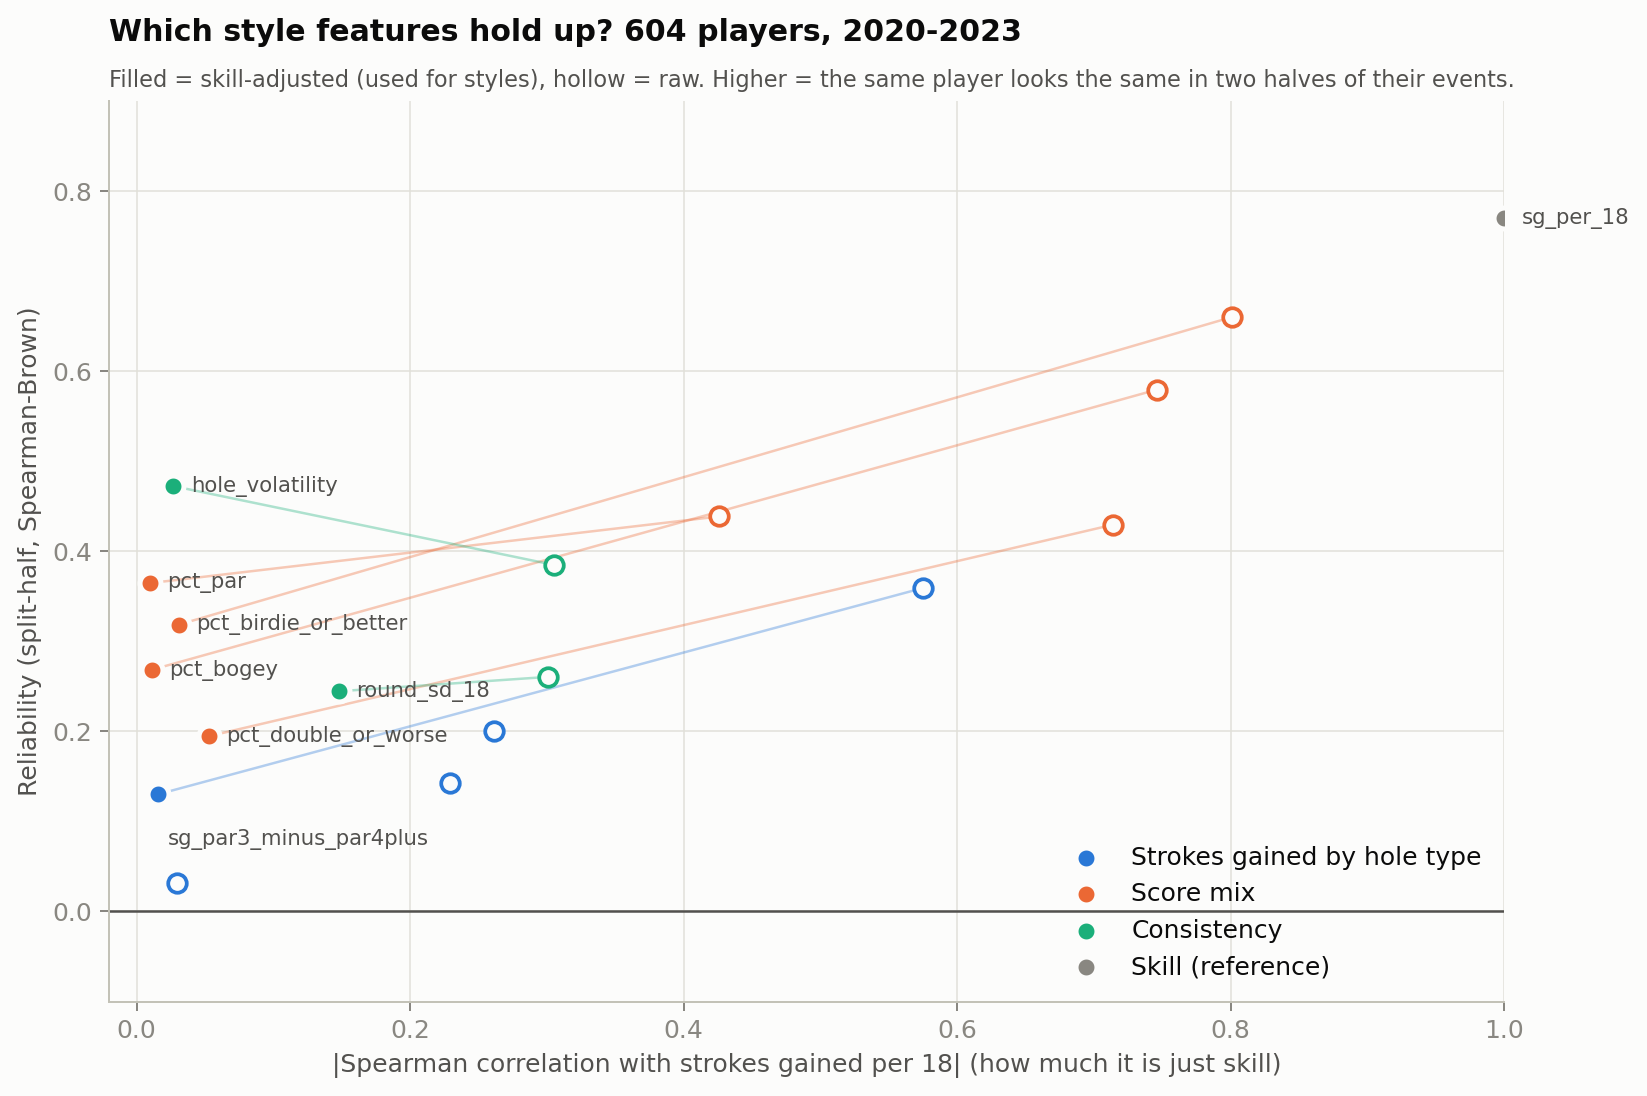
\includegraphics[width=0.66\textwidth]{figures/eda_feature_reliability.png}
\caption{Split-half reliability of each profile feature against its correlation with skill ($|\rho|$ with strokes gained per 18). Hollow points are raw features, filled points are the skill-adjusted versions, and lines connect each pair. Features that are both reliable and not just skill would sit in the top left.}
\label{fig:reliability}
\end{figure}

\subsection{Clustering and validation}

I clustered the ten standardized style features with K-means and Gaussian mixture models (GMM), comparing them with silhouette scores and BIC. I then checked how stable the two-cluster solution is: whether K-means and the GMM agree, whether it changes with a stricter minimum-data threshold or under bootstrap resampling, and whether PCA shows separate groups or one continuous cloud. Rating and strokes gained per 18 aren't clustering inputs. I only use them afterwards to check whether the clusters are just picking up skill.

% ---------------------------------------------------------------------------
\section{Results so far}


\subsection{Two clusters: steady and volatile}

Silhouette scores were low for every number of clusters I tried, so I focused on the simplest split, two clusters. Figure~\ref{fig:centroids} shows the cluster means. Compared with players at a similar performance level, one cluster makes fewer pars and birdies and more bogeys and doubles or worse, and has more volatile hole scores. The other cluster is the opposite. Both clusters are near zero on the hole type features, so what separates them is how consistently players score, not which kinds of holes they do well on. I'll call cluster 0 ``volatile'' and cluster 1 ``steady''.

\begin{figure}[t]
\centering
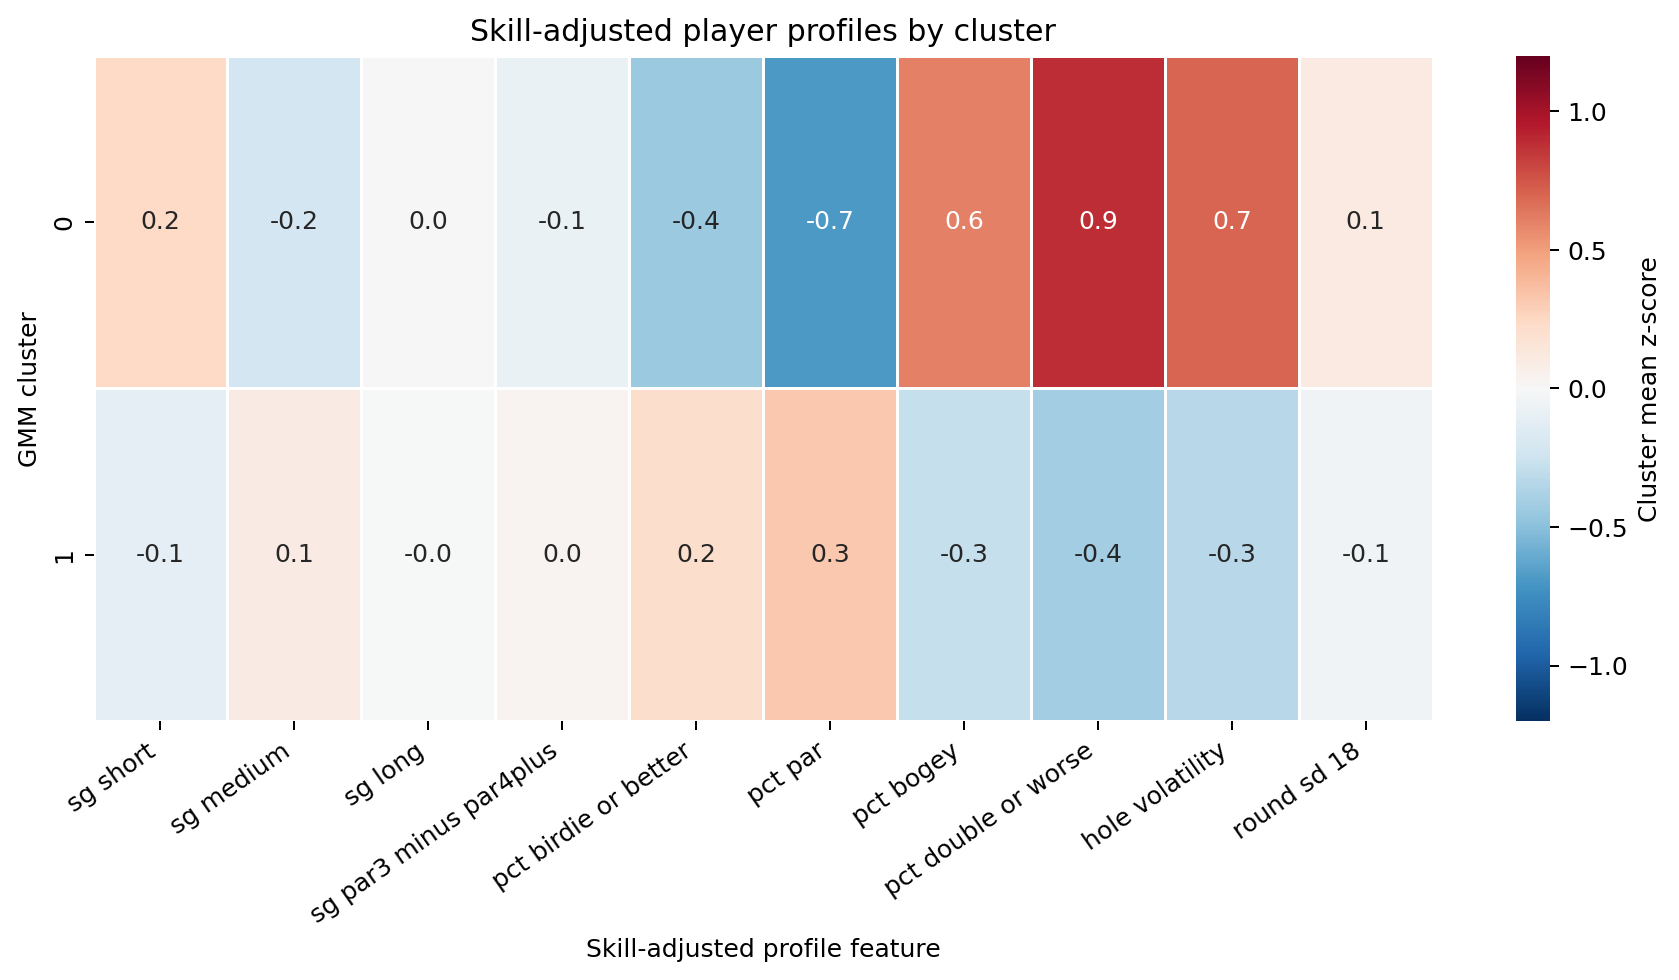
\includegraphics[width=0.78\textwidth]{figures/clustering_profile_centroids.png}
\caption{Mean of each standardized, skill-adjusted profile feature for the two GMM clusters. Cluster 0 ($n = 194$) has more bogeys and doubles and fewer pars than its skill level would predict. Cluster 1 ($n = 410$) is the reverse. The strokes gained by hole type columns barely differ.}
\label{fig:centroids}
\end{figure}

The clusters aren't independent of skill, though (Figure~\ref{fig:rating}). The volatile cluster has a higher median rating (915 vs.\ 888), but lower median strokes gained per 18 (0.66 vs.\ 0.89). At a given rating, volatile players tend to gain fewer strokes on the field than steady ones. One explanation is that a volatile player's good rounds keep their rating up even though their typical round is worse. Another is field strength. Higher-rated players often share a layout with stronger divisions, and strokes gained is measured against whoever else played that layout. I can't separate these two yet, but either way I don't think the clusters can be described as purely about style.

\begin{figure}[t]
\centering
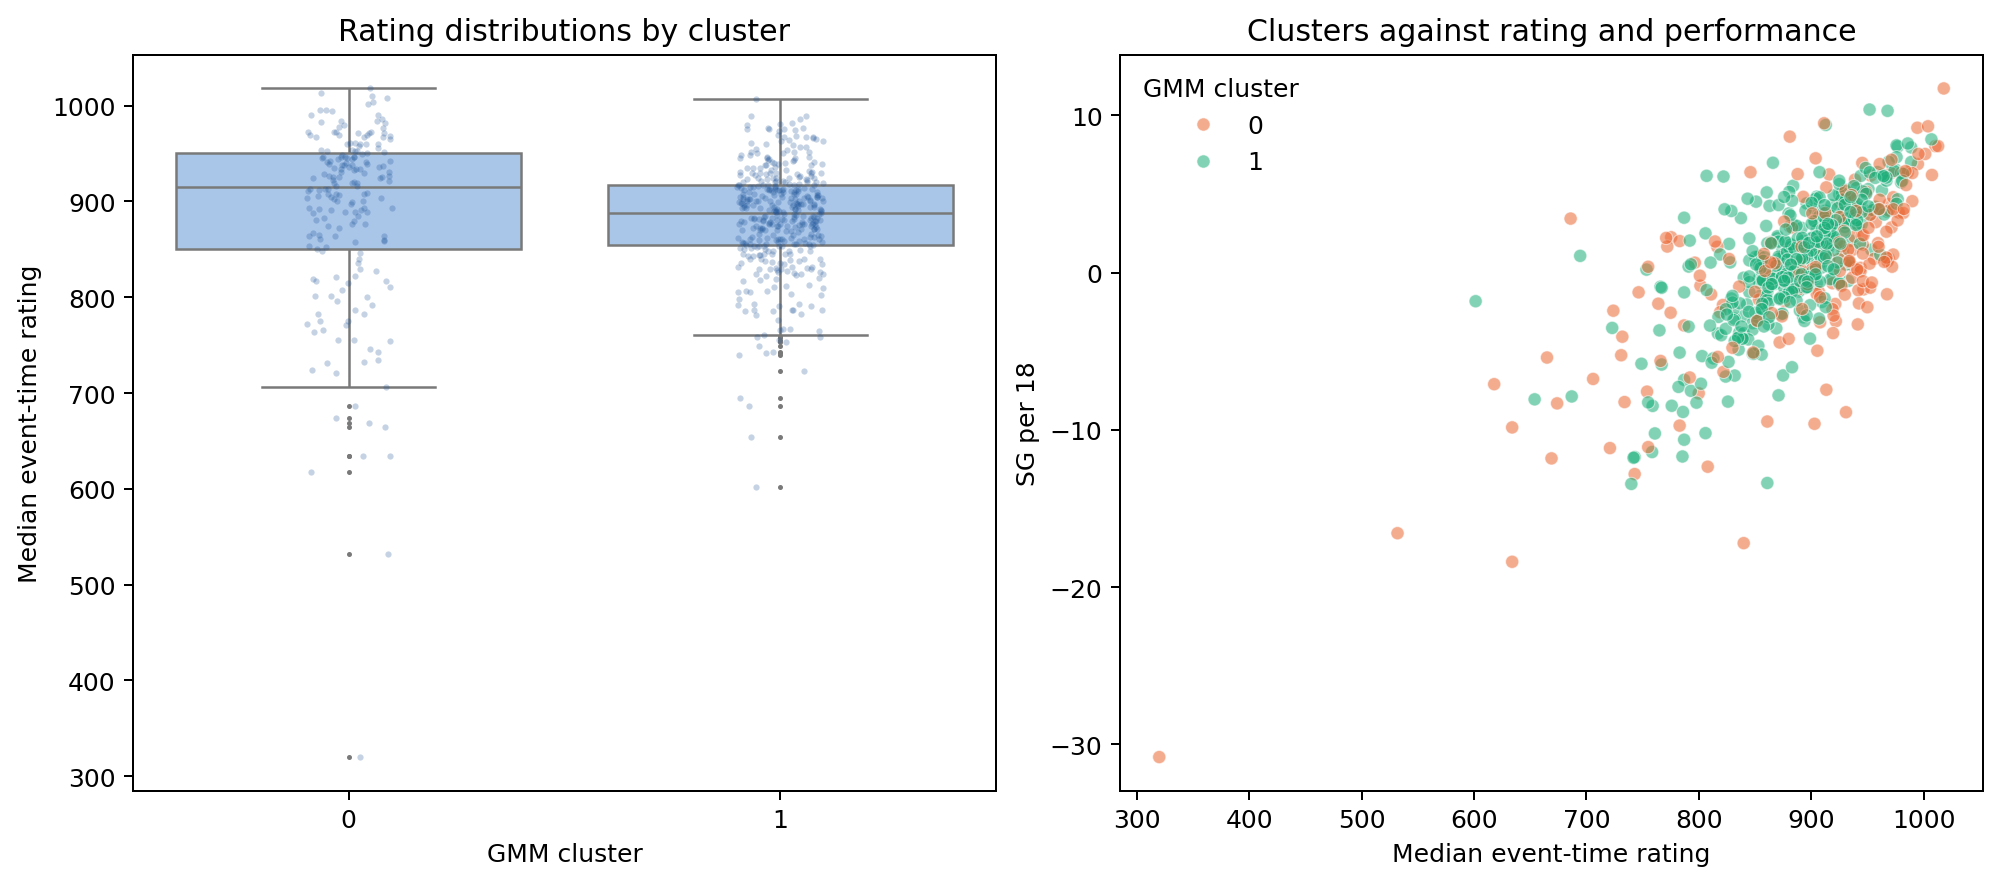
\includegraphics[width=0.85\textwidth]{figures/clustering_rating_comparison.png}
\caption{Left: median event-time rating by cluster. Right: strokes gained per 18 against rating, colored by cluster. Both clusters cover the full rating range, but at a given rating the volatile players (cluster 0) tend to sit below the steady players (cluster 1).}
\label{fig:rating}
\end{figure}

\subsection{Robustness}

The two-cluster split mostly holds up when I switch algorithms or require more data per player, and it separates more cleanly when I cluster on only the more reliable score mix and consistency features. The bootstrap is less reassuring, since some resamples give quite different splits. In a PCA projection the two clusters look like two halves of one cloud, not two separate groups. I'm still working through these checks and will report them in full in the final report.

Overall, players do seem to differ in how consistently they score, even after accounting for skill. That difference is moderately reliable and gives a two-cluster split that mostly holds up. But the split looks like a cut through a continuum. It's still tied to the gap between rating and performance, and it says very little about hole type preferences. Right now I think the data support a steady-versus-volatile dimension, not a set of distinct archetypes.

% ---------------------------------------------------------------------------
\section{Discussion}

\subsection{How the project has gone}

Data collection went better than I expected. In the proposal I was worried that older events wouldn't have hole by hole scores and that I might have to fall back on round-level features. I ended up scraping every DGVT event from 2019 to 2026, and 2020 onward has almost complete hole level coverage. Splitting the processing into separate scripts for combining seasons, checking data quality and building features also made it easy to change definitions as I went. For example, when I decided to keep hole length and field difficulty as separate features, I only had to change the feature script and rerun it.

The clustering has been less clean than I hoped. In the proposal I was picturing something like the basketball paper [2], where clustering found 13 player types in place of the 5 traditional positions. That isn't what I'm seeing. The reliability check ended up being more informative than the clustering itself. It showed that the hole type features, which are what I originally thought of as ``style'', are mostly noise at this sample size, since most players have fewer than 200 holes in the profile window. I also underestimated how hard it is to remove skill. Even after taking residuals on strokes gained per 18, the clusters still line up with the gap between rating and strokes gained.

My proposal's contingency plan did list both of these possibilities (``the clusters just recover skill'' and ``there aren't distinct groups''), with continuous style dimensions as the fallback. That fallback is now my main plan. The minimum viable project still looks doable: the player $\times$ hole table, strokes gained, style profiles and a validated clustering are done, and the style $\times$ hole type model and the prediction comparison are what's left.

\subsection{Limitations and risks}

\begin{itemize}
  \item \emph{Selection.} Players choose which events, and so which courses, they play. A profile partly reflects that course mix and the player's division. Player effects in the explanatory model should absorb some of this, and the results only apply to players who showed up.
  \item \emph{Field strength.} Strokes gained is measured against whoever played the same layout, so it isn't fully comparable between layouts with stronger and weaker fields. The score mix features have a related problem, since they're measured against par: players on harder layouts make more bogeys at the same strokes gained, and higher-rated players tend to play the longer tees. Adjusting for strokes gained per 18 doesn't remove this, and I think it's part of what's going on in Figure~\ref{fig:rating}.
  \item \emph{Sample size.} The 2-event threshold keeps 57\% of eligible players, but a lot of them are close to the minimum, so their profiles are noisy. The stricter threshold gives similar clusters, but it doesn't make the hole type features any more reliable.
  \item \emph{Skill.} Rating and strokes gained per 18 are strongly related, and adjusting for one still leaves structure related to the other.
  \item \emph{Unstable labels.} Given the low silhouette scores and the bootstrap results, I don't think individual cluster labels should be read as fixed player identities.
\end{itemize}

\subsection{Plan for the rest of the semester}

I'm keeping the proposal's structure and timeline. The main change is that in the later models I'll mainly use a continuous volatility score for style, and use the two-cluster label as a secondary, easier-to-read version.

\begin{table}[H]
\centering
\footnotesize
\setlength{\tabcolsep}{4pt}
\renewcommand{\arraystretch}{0.92}
\begin{tabularx}{\textwidth}{@{}p{1.25cm}Y>{\raggedright\arraybackslash}p{4.2cm}@{}}
\toprule
\textbf{Week of} & \textbf{Work} & \textbf{Deliverable} \\
\midrule
Nov 2  & Finish stability checks (season to season: 2020--21 vs.\ 2022--23); define a continuous style score (PC1 or a volatility index) and compare it with the cluster labels; adjust strokes gained for field strength &
  Final style dimensions \\
Nov 9  & Mixed-effects model on held-out 2024--2026 scores: strokes gained $\sim$ hole type $\times$ style + difficulty, with player and layout-round-hole random effects &
  Explanatory results \\
Nov 16 & Predict score category (birdie or better, par, bogey, double or worse) on held-out events from rating and difficulty, then with style added; compare log loss and calibration &
  Predictive results \\
Nov 23 & Buffer (Thanksgiving); README, license and docs; stretch goal: does a bad hole carry over to the next one? &
  Clean up repo \\
Nov 30 & Write the final report & Report draft \\
Dec 7  & Revise and present &
  \textbf{Report (Dec 8), presentation (Dec 9)} \\
\bottomrule
\end{tabularx}
\end{table}

The results so far change two parts of this plan. First, in the explanatory model I want to test the volatility dimension against field difficulty, not just hole length. My guess is that steady players gain the most on holes where a lot of the field makes big numbers, more than on long holes specifically. Second, the prediction comparison is where I'll find out whether style is a real property of a player. If adding the volatility score improves held-out predictions of double bogey or worse, the category where the two clusters differ most, that's good evidence it's real. If it doesn't help, I'll report that the profile differences are descriptive variation and not a stable style.

\textbf{Code and data.} The project repository is \url{https://github.com/lcohenwanis/disc-golf-play-styles-ds2-2026}. The scraper and processing scripts are in \texttt{dgvt\_styles/}, and the analysis is in two notebooks: \texttt{notebooks/dgvt-eda.ipynb} (features, profiles, reliability) and \texttt{notebooks/clustering\_analysis.ipynb} (clustering and stability checks). All of the figures here come from those notebooks.

% ---------------------------------------------------------------------------
{\footnotesize
\textbf{References.}
[1] M.~Broadie. Assessing golfer performance on the PGA TOUR.
\emph{Interfaces}, 42(2):146--165, 2012.
[2] M.~Alagappan. From 5 to 13: Redefining the positions in basketball.
\emph{MIT Sloan Sports Analytics Conference}, 2012.
}

\end{document}
